\documentclass[12pt]{article}
\usepackage{lecture}
\usepackage{html}
\usepackage{graphics}
\usepackage{epstopdf}

\newcommand{\copyrightYears}{2004-2012}

\title{Analyzing the genetic structure of populations: individual assignment}

\begin{document}

\maketitle

\thispagestyle{first}

\section*{Introduction}

In the last 10-12 years a different approach to the analysis of
genetic structure has emerged: analysis of individual
assignment.\index{individual assignment} Although the implementation
details get a little hairy, the basic idea is fairly simple. Suppose
we have genetic data on a series of individuals. Label the data we
have for each individual $x_i$. Suppose that all individuals belong to
one of $K$ populations and let the genotype frequencies in population
$k$ be represented by $\gamma_k$. Then the likelihood that individual
$i$ comes from population $k$ is just
\[
\mbox{P}(i|k) = \frac{\mbox{P}(x_i|\gamma_k)}{\sum_k
  \mbox{P}(x_i|\gamma_k)} \quad .
\]
So if we can specify prior probabilities for $\gamma_k$, we can use
Bayesian methods to estimate the posterior probability that individual
$i$ belongs to population $k$, and we can associate that assignment
with some measure of its reliability.\footnote{You can find details
  in~\cite{Pritchard-etal-2000}.}

\section*{Applying assignment to understand invasions}

We'll use {\tt Structure} to assess whether cultivated genotypes of
{\it Berberis thunbergii\/} contribute to ongoing invasions in
Connecticut and
Massachusetts~\cite{Lubell-etal-2008}.\index{individual assignment!application} The first problem is to determine what $K$
to use, because $K$ doesn't necessarily have to equal the number of
populations we sample from. Some populations may not be distinct from
one another. There are a couple of ways to estimate $K$. The most
straightforward is to run the analysis for a range of plausible
values, repeat it 10-20 times for each value, calculate the mean ``log
probability of the data'' for each value of $K$, and pick the value of
$K$ that is the biggest, i.e., the least
negative~(Table~\ref{table:berberis-k}). For the barberry data, $K=3$
is the obvious choice.

\begin{table}
\begin{center}
\begin{tabular}{cc}
\hline\hline
K & Mean L(K) \\
\hline
2 & -2553.2 \\
3 & {\bf -2331.9} \\
4 & -2402.9 \\
5 & -2476.3 \\
\hline
\end{tabular}
\end{center}
\caption{Mean log probability of the data for $K=2,3,4,5$ in the {\it
    Berberis thunbergii\/} data~(adapted
  from~\cite{Lubell-etal-2008}).}\label{table:berberis-k}
\end{table}

Having determined that the data support $K=3$, the results of the
analysis are displayed in Figure~\ref{fig:lubell-structure}. Each
vertical bar corresponds to an individual in the sample, and the
proportion of each bar that is of a particular color tells us the
posterior probability that the individual belongs to the cluster with
that color.

\begin{figure}
\resizebox{\textwidth}{!}{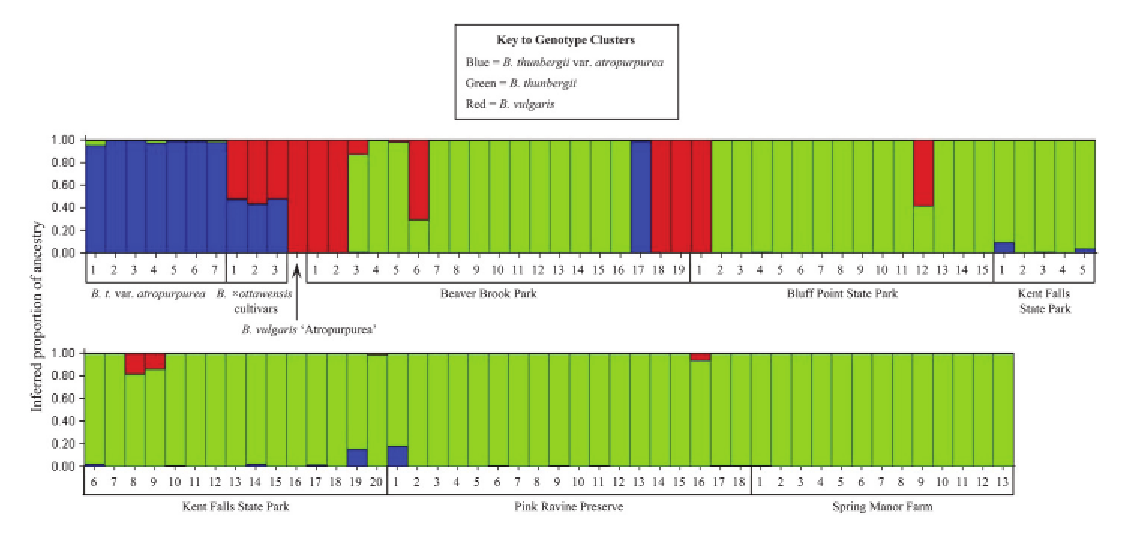
\includegraphics{lubell-structure.eps}}
\caption{Analysis of AFLP data from {\it Berberis
    thunbergii}~\cite{Lubell-etal-2008}.}\label{fig:lubell-structure} 
\end{figure}

Figure~\ref{fig:lubell-structure} may not look terribly informative,
but actually it is. Look at the labels beneath the figure. You'll see
that with te exception of individual 17 from Beaver Brook Park, all
the of the individuals that are solid blue are members of the
cultivated {\it Berberis thunbergii\/} var. {\it atropurpurea}. The
solid red bar corresponds to {\it Berberis thunbergii\/}
'Atropurpurea', another modern cultivar. You'll notice that
individuals 1, 2, 18, and 19 from Beaver Brook Park and individual 1
from Bluff Point State Park fall into the same genotypic cluster as
this cultivar. {\it Berberis $\times$ottawensis} is a hybrid cultivar
whose parents are {\it Berberis thunbergii\/} and {\it Berberis
  vulgaris\/}, so it makes sense that individuals of this cultivar
would be half blue and half red. The solid green bars are feral
individuals from long-established populations. Notice that the
cultivars are distinct from all but a few of the individuals in the
long-established feral populations, suggesting that contemporary
cultivars are doing relatively little to maintain the invasion in
areas where it is already established.

\bibliography{popgen}
\bibliographystyle{plain}

\ccLicense

\end{document}
